\documentclass[12pt]{article}
\usepackage[a4paper, portrait, margin=1cm, right=1cm]{geometry}
\usepackage{fontspec}
\usepackage[fleqn]{amsmath}
\usepackage{setspace}
\usepackage{graphicx}
\usepackage{ulem}
\graphicspath{./graphics/}
\setmainfont[Ligatures=TeX]{Linux Libertine}

\title{Физика. ДЗ-2. Механика. Динамика}
\author{Студент группы 2305 Александр Макурин}
\date{08.12.2022}

\begin{document}

\maketitle

\begin{sloppypar}
    \setstretch{1.8}

    \section*{Задача 1.}
    $G = 6.67430(15) \cdot 10^{-11} \dfrac{\text{м}^3}{\text{с}^2\text{кг}}$ — гравитационная постоянная \\
    $M = 5.9742 \cdot 10^{24}$ кг — масса Земли \\
    $R = 6.378 \cdot 10^6$ м — радиус Земли \\
    $R_{ZS} = 1.4959787 \cdot 10^{11}$ м — среднее расстояние от Земли до Солнца \\
    $M_S = 1.98892 \cdot 10^{30}$ кг — масса Солнца
    \[
        \dfrac{mV_1^2}{R} = G\dfrac{mM}{R^2} \Rightarrow V_1 = \sqrt{\dfrac{GM}{R}}
    \]
    \[
        \dfrac{mV_2^2}{2} - G\dfrac{mM}{R} = 0 \Rightarrow V_2 = \sqrt{2\dfrac{GM}{R}} = V_1\sqrt2
    \]
    Для выхода за пределы солнечной системы ракете требуется:
    \begin{enumerate}
        \item{Преодолеть притяжение Земли}
        \item{Преодолеть притяжение Солнца, с учётом того, что Земля уже движется с первой космической относительно Солнца}
    \end{enumerate}
    \[
        V_S = \sqrt{\dfrac{2GM_S}{R_{ZS}}}
    \]
    $V_S$ - вторая космическая (для выхода за пределы Солнечной Системы) скорость ракеты, стартующей с орбиты Земли, относительно Солнца, $R_{ZS}$ - расстояние от Земли до Солнца, $M_S$ - масса Солнца
    \[
        V_Z = \sqrt{\dfrac{GM_S}{R_{ZS}}}
    \]
    $V_Z$ - первая космическая для Земли относительно Солнца
    \[
        V_{RZ} = V_S - V_Z = V_Z(\sqrt2 - 1)
    \]
    $V_{RZ}$ - вторая космическая (для выхода за пределы Солнечной Системы) скорость ракеты, стартующей с орбиты Земли, относительно Земли
    \[
        \dfrac{mV_3^2}{2} = \dfrac{mV_2^2}{2} + \dfrac{mV_{RZ}^2}{2} \Rightarrow V_3 = \sqrt{V_2^2 + V_{RZ}^2} = \sqrt{V_2^2 + V_Z^2(\sqrt2 - 1)^2}
    \]
    \[
        V_3 = \sqrt{V_2^2 + V_Z^2(\sqrt2 - 1)^2}
    \]
    \fbox{
        Ответ:
        \[
            \left|\begin{array}{lcl}
                V_1 = & \sqrt{\dfrac{GM}{R}}               & = 7.906795973 \cdot 10^3 \  \dfrac{\text{м}}{\text{с}} \\
                V_2 = & V_1\sqrt2                          & = 1.118189810 \cdot 10^4 \  \dfrac{\text{м}}{\text{с}} \\
                V_3 = & \sqrt{V_2^2 + V_Z^2(\sqrt2 - 1)^2} & = 1.665175691 \cdot 10^4 \  \dfrac{\text{м}}{\text{с}}
            \end{array}\right.
        \]
    }

    \section*{Задача 2.}
    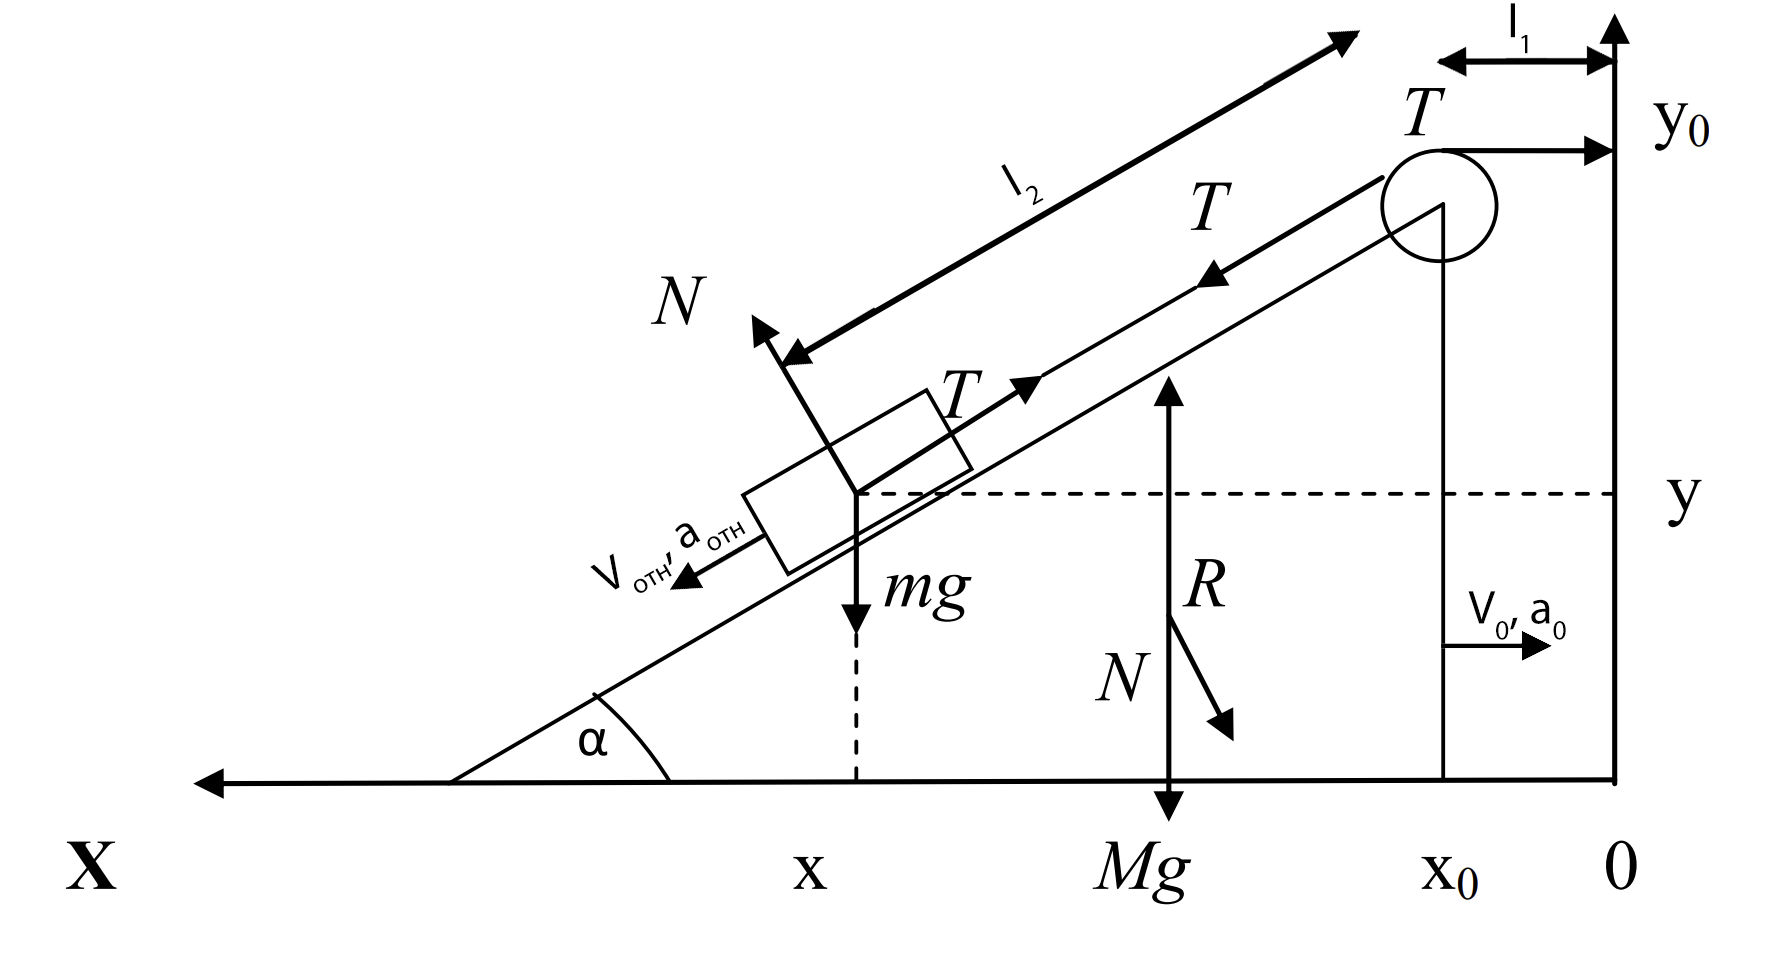
\includegraphics[width=0.8\textwidth]{graphics/task_02.png}
    \[
        \dfrac{dl_1}{dt} = V_{\text{отн}}
    \]
    \[
        \dfrac{dl_2}{dt} = -V_0
    \]
    \[
        l_1 + l_2 = const \Rightarrow V_\text{отн} = V_0 \Rightarrow a_\text{отн} = a_0
    \]
    По третьему закону Ньютона:
    \[
        \begin{array}{l}
            T - mg\sin\alpha = m(a_0\cos\alpha - a_\text{отн}) = Ma_0(\cos\alpha - 1) \\
            N - Ma\cos\alpha = m(-a_0\sin\alpha)                                      \\
            N\sin\alpha + T(1 - \cos\alpha) = Ma_0                                    \\
            N = \dfrac{Ma_0 - T(1 - \cos\alpha)}{\sin\alpha}
        \end{array}
    \]
    \[
        \begin{array}{l}
            T = mg\sin\alpha - ma_0(1-\cos\alpha)                                                \\
            Ma_0 - mgsin\alpha + ma_0 - 2ma_0\cos\alpha + ma_0\cos^2\alpha +ma_0\sin^2\alpha = 0 \\
            (M + 2m(1- \cos\alpha))a_0 = mg\sin\alpha                                            \\
            a_0 = g\dfrac{\sin\alpha}{\dfrac{M}{m} + 2(1 - \cos\alpha)} \Rightarrow A_x = -a_0 \Rightarrow A_x = -g\dfrac{\sin\alpha}{\dfrac{M}{m} + 2(1 - \cos\alpha)}
        \end{array}
    \]

    \fbox{Ответ: $A_x = -g\dfrac{\sin\alpha}{\dfrac{M}{m} + 2(1 - \cos\alpha)}$}

    \section*{Задача 4.}
    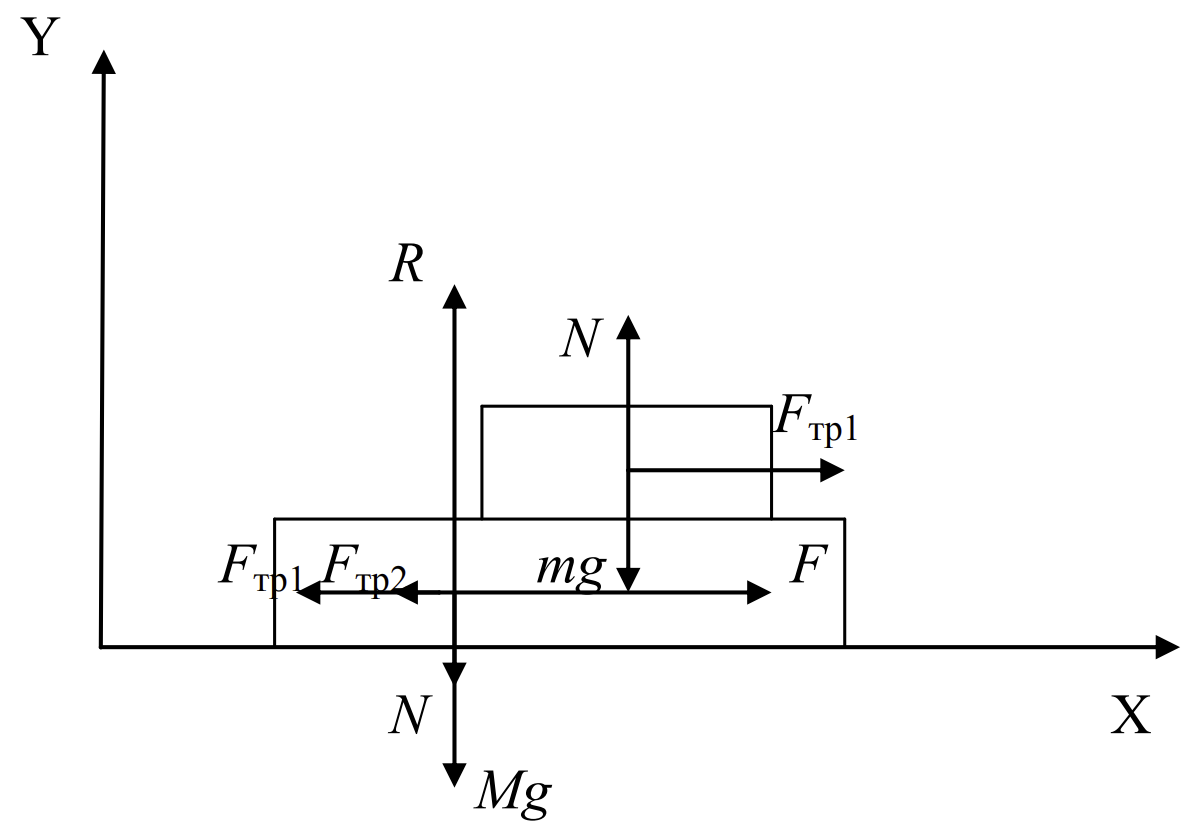
\includegraphics[width=0.8\textwidth]{graphics/task_04.png}

    \[
        \begin{array}{l}
            N_1 = mg                               \\
            R = N_1 + Mg = g(m + M)                \\
            F - F_{\text{тр1}} - F_\text{тр2} = Ma \\
            F_\text{тр1} = ma
        \end{array}
    \]
    Если $F_\text{тр1} \geq \mu_1mg$, начнётся скольжение $\Rightarrow a = \mu_1g$
    \[
        \begin{array}{ll}
            F & = \mu_1N_1 + \mu_2R + Ma = \mu_1mg + \mu_2g(m + M) + \mu_1Mg = \mu_1mg + \mu_1Mg + \mu_2mg + \mu_2Mg = \\
              & = g(\mu_1(m + M) + \mu_2(m + M)) = g(\mu_1 + \mu_2)(m + M)
        \end{array}
    \]
    \fbox{Ответ: $F \geq g(\mu_1 + \mu_2)(m + M) = 10(0.25 + 0.5)(2 + 1) = 22.5$ Н}

\end{sloppypar}
\end{document}
